\documentclass[aspectratio=169,12pt]{beamer}
\usepackage[utf8]{inputenc}
\usepackage{amsmath, amssymb}
\usepackage{booktabs}
\usepackage{colortbl}
\usepackage{hyperref}
\usepackage{makecell}
\usepackage{ragged2e}
\usepackage{tikz}
\usetikzlibrary{arrows.meta, positioning, shapes.geometric, calc, tikzmark, shapes.misc, fit, decorations.pathreplacing, matrix}
\usepackage{tcolorbox}
\usepackage{array}
\usepackage{listings}
\usepackage{pgfkeys}
\usepackage[normalem]{ulem} 
\usetheme{Madrid}

% Custom colors - consolidated
\definecolor{correctgreen}{RGB}{0,150,0}
\definecolor{incorrectred}{RGB}{200,0,0}
\definecolor{counterblue}{RGB}{70,130,255}
\definecolor{highlightyellow}{RGB}{255,230,100}
\definecolor{lightblue}{RGB}{200,230,250}
\definecolor{darkblue}{RGB}{0,100,200}
\definecolor{highlightorange}{RGB}{255,200,100}

% Define asmcode command for assembly code formatting
\newcommand{\asmcode}[1]{\tiny\texttt{#1}}

% Commands for highlighting entries
\newcommand{\oldentry}[1]{~#1}
\newcommand{\newentrya}[1]{\colorbox{highlightyellow}{#1}}
\newcommand{\newentryb}[1]{\colorbox{highlightorange}{#1}}
\newcommand{\srcentrya}[1]{\colorbox{highlightyellow!30}{#1}}
\newcommand{\srcentryb}[1]{\colorbox{highlightorange!30}{#1}}

\pgfkeys{
    /OOO/.is family, /OOO,
    default/.style = {
        % RAT registers
        R1 = {}, R2 = {}, R3 = {}, R4 = {}, R5 = {},
        R6 = {}, R7 = {}, R8 = {}, R9 = {}, R10 = {},
        % ROB cells (2 columns x 9 rows)
        rob01 = {}, rob02 = {},
        rob11 = {}, rob12 = {},
        rob21 = {}, rob22 = {},
        rob31 = {}, rob32 = {},
        rob41 = {}, rob42 = {},
        rob51 = {}, rob52 = {},
        rob61 = {}, rob62 = {},
        rob71 = {}, rob72 = {},
        rob81 = {}, rob82 = {},
        % ROB left markers
        robleft0 = {}, robleft1 = {}, robleft2 = {},
        robleft3 = {}, robleft4 = {}, robleft5 = {},
        robleft6 = {}, robleft7 = {}, robleft8 = {},
        % IDQ cells
        idq1 = {}, idq2 = {},
        % RS cells
        rs1 = {}, rs2 = {}, rs3 = {}, rs4 = {}, rs5 = {}, rs6 = {},
        % RS markers
        rsmark1 = {}, rsmark2 = {}, rsmark3 = {}, rsmark4 = {}, rsmark5 = {}, rsmark6 = {},
        % MOB cells
        mob1 = {}, mob2 = {},
        % MOB markers
        mobmark1 = {}, mobmark2 = {},
        % Execute cells
        exec1 = {}, exec2 = {},
        % Retire cells
        ret1 = {}, ret2 = {},
        % Retire markers
        retmark1 = {}, retmark2 = {},
        % Code highlighting (line numbers to highlight)
        highlight1 = 0, highlight2 = 0,
        % Show code flag
        showcode = 1,
        % Number of rows/cols (for iteration purposes)
        rob rows = 9,
        idq rows = 2,
        rs rows = 6,
        mob rows = 2,
        execute rows = 2,
        retire cols = 2
    },
    % RAT mappings
    R1/.estore in = \prfOne,
    R2/.estore in = \prfTwo,
    R3/.estore in = \prfThree,
    R4/.estore in = \prfFour,
    R5/.estore in = \prfFive,
    R6/.estore in = \prfSix,
    R7/.estore in = \prfSeven,
    R8/.estore in = \prfEight,
    R9/.estore in = \prfNine,
    R10/.estore in = \prfTen,
    % ROB cell contents
    rob01/.estore in = \robZeroOne, rob02/.estore in = \robZeroTwo,
    rob11/.estore in = \robOneOne, rob12/.estore in = \robOneTwo,
    rob21/.estore in = \robTwoOne, rob22/.estore in = \robTwoTwo,
    rob31/.estore in = \robThreeOne, rob32/.estore in = \robThreeTwo,
    rob41/.estore in = \robFourOne, rob42/.estore in = \robFourTwo,
    rob51/.estore in = \robFiveOne, rob52/.estore in = \robFiveTwo,
    rob61/.estore in = \robSixOne, rob62/.estore in = \robSixTwo,
    rob71/.estore in = \robSevenOne, rob72/.estore in = \robSevenTwo,
    rob81/.estore in = \robEightOne, rob82/.estore in = \robEightTwo,
    % ROB left markers
    robleft0/.estore in = \robLeftZero,
    robleft1/.estore in = \robLeftOne,
    robleft2/.estore in = \robLeftTwo,
    robleft3/.estore in = \robLeftThree,
    robleft4/.estore in = \robLeftFour,
    robleft5/.estore in = \robLeftFive,
    robleft6/.estore in = \robLeftSix,
    robleft7/.estore in = \robLeftSeven,
    robleft8/.estore in = \robLeftEight,
    % IDQ cell contents
    idq1/.estore in = \idqOne,
    idq2/.estore in = \idqTwo,
    % RS cell contents
    rs1/.estore in = \rsOne,
    rs2/.estore in = \rsTwo,
    rs3/.estore in = \rsThree,
    rs4/.estore in = \rsFour,
    rs5/.estore in = \rsFive,
    rs6/.estore in = \rsSix,
    % RS markers
    rsmark1/.estore in = \rsMarkOne,
    rsmark2/.estore in = \rsMarkTwo,
    rsmark3/.estore in = \rsMarkThree,
    rsmark4/.estore in = \rsMarkFour,
    rsmark5/.estore in = \rsMarkFive,
    rsmark6/.estore in = \rsMarkSix,
     % MOB cell contents
    mob1/.estore in = \mobOne,
    mob2/.estore in = \mobTwo,
    % MOB markers
    mobmark1/.estore in = \mobMarkOne,
    mobmark2/.estore in = \mobMarkTwo,
    % Execute cell contents
    exec1/.estore in = \execOne,
    exec2/.estore in = \execTwo,
    % Retire cell contents
    ret1/.estore in = \retOne,
    ret2/.estore in = \retTwo,
    % Retire markers
    retmark1/.estore in = \retMarkOne,
    retmark2/.estore in = \retMarkTwo,
    % Code highlighting
    highlight1/.estore in = \highlightOne,
    highlight2/.estore in = \highlightTwo,
    showcode/.estore in = \showCode,
    % Store row/col counts
    rob rows/.estore in = \robRows,
    idq rows/.estore in = \idqRows,
    rs rows/.estore in = \rsRows,
    mob rows/.estore in = \mobRows,
    execute rows/.estore in = \executeRows,
    retire cols/.estore in = \retireCols,
}

\newcommand{\OOODiagramKV}[1][]{%
    % Set defaults and process keys
    \pgfkeys{/OOO,default,#1}%
    %
    \begin{tikzpicture}[
        cell/.style={draw, minimum width=0.8cm, minimum height=0.35cm},
        nocell/.style={minimum width=0.8cm, minimum height=0.35cm},
        roundbox/.style={draw, ellipse, minimum width=3cm, minimum height=1.5cm},
        dashedbox/.style={draw, dashed, rectangle, minimum width=3cm, minimum height=1cm},
        codebox/.style={draw, rectangle, fill=correctgreen!20, minimum width=3.0cm}
    ]
    %
    % RAT (Register Alias Table)
    \matrix[matrix of nodes, 
            nodes={cell, anchor=center,         
            minimum height=4mm,
            text height=1ex,
            text depth=0.25ex},
            column sep=-\pgflinewidth,
            row sep=-\pgflinewidth,
            inner sep=0pt,
            label={left:\textbf{RAT}},
            ampersand replacement=\&] (rat) {
        \scriptsize R1 \& \scriptsize \prfOne \\
        \scriptsize R2 \& \scriptsize \prfTwo \\
        \scriptsize R3 \& \scriptsize \prfThree \\
        \scriptsize R4 \& \scriptsize \prfFour \\
        \scriptsize R5 \& \scriptsize \prfFive \\
        \scriptsize R6 \& \scriptsize \prfSix \\
        \scriptsize R7 \& \scriptsize \prfSeven \\
        \scriptsize R8 \& \scriptsize \prfEight \\
        \scriptsize R9 \& \scriptsize \prfNine \\
        \scriptsize R10 \& \scriptsize \prfTen \\
    };
    %
    % ROB (Reorder Buffer) - 3 columns (left marker, instruction, status)
    \matrix[matrix of nodes,
            column sep=-\pgflinewidth,
            row sep=-\pgflinewidth,
            inner sep=0pt,
            label={left:\textbf{ROB}},
            below=0.2cm of rat,
            anchor=north,
            nodes in empty cells,
            nodes={cell, align=left},
            column 1/.append style={nodes={text width=0.5cm, minimum height=4mm, text height=1ex, text depth=0.25ex}},
            column 2/.append style={nodes={text width=3cm, minimum height=4mm, text height=1ex, text depth=0.25ex}},
            column 3/.append style={nodes={text width=0.8cm, minimum height=4mm, text height=1ex, text depth=0.25ex}},
            ampersand replacement=\&
        ] (rob) {
    |[cell]| \scriptsize \robLeftZero \& |[cell]| \scriptsize \robZeroOne  \& |[cell]| \scriptsize \robZeroTwo \\
    |[cell]| \scriptsize \robLeftOne  \& |[cell]| \scriptsize \robOneOne   \& |[cell]| \scriptsize \robOneTwo \\
    |[cell]| \scriptsize \robLeftTwo  \& |[cell]| \scriptsize \robTwoOne   \& |[cell]| \scriptsize \robTwoTwo \\
    |[cell]| \scriptsize \robLeftThree\& |[cell]| \scriptsize \robThreeOne \& |[cell]| \scriptsize \robThreeTwo \\
    |[cell]| \scriptsize \robLeftFour \& |[cell]| \scriptsize \robFourOne  \& |[cell]| \scriptsize \robFourTwo \\
    |[cell]| \scriptsize \robLeftFive \& |[cell]| \scriptsize \robFiveOne  \& |[cell]| \scriptsize \robFiveTwo \\
    |[cell]| \scriptsize \robLeftSix  \& |[cell]| \scriptsize \robSixOne   \& |[cell]| \scriptsize \robSixTwo \\
    |[cell]| \scriptsize \robLeftSeven\& |[cell]| \scriptsize \robSevenOne \& |[cell]| \scriptsize \robSevenTwo \\
    |[cell]| \scriptsize \robLeftEight\& |[cell]| \scriptsize \robEightOne \& |[cell]| \scriptsize \robEightTwo \\
    };
    %
    % IDQ (Instruction Decode Queue) - 2 rows
    \matrix[matrix of nodes,
            row sep=-\pgflinewidth,
            inner sep=0pt,
            label={right:\textbf{IDQ}},
            right=3cm of rat.north east,
            anchor=north west,
            nodes={cell, text width=3cm, align=left},
            ampersand replacement=\&] (idq) {
        |[cell]| \scriptsize \idqOne \\
        |[cell]| \scriptsize \idqTwo \\
    };
    %
    % RS (Reservation Station) - 6 rows
    \matrix[matrix of nodes,
            row sep=-\pgflinewidth,
            inner sep=0pt,
            label={above:\textbf{RS}},
            below=0.6cm of idq.south, anchor=north,
            nodes={cell, text width=3cm, align=left},
            ampersand replacement=\&] (rs) {
        |[cell]| \scriptsize \rsOne \\
        |[cell]| \scriptsize \rsTwo \\
        |[cell]| \scriptsize \rsThree \\
        |[cell]| \scriptsize \rsFour \\
        |[cell]| \scriptsize \rsFive \\
        |[cell]| \scriptsize \rsSix \\
    };
    %
    % Add markers for RS rows (on the right)
    \coordinate (rsmarker1) at ($(rs-1-1.east)+(0.2,0)$);
    \node[anchor=west, inner sep=1pt, font=\tiny] at (rsmarker1) {\rsMarkOne};
    \coordinate (rsmarker2) at ($(rs-2-1.east)+(0.2,0)$);
    \node[anchor=west, inner sep=1pt, font=\tiny] at (rsmarker2) {\rsMarkTwo};
    \coordinate (rsmarker3) at ($(rs-3-1.east)+(0.2,0)$);
    \node[anchor=west, inner sep=1pt, font=\tiny] at (rsmarker3) {\rsMarkThree};
    \coordinate (rsmarker4) at ($(rs-4-1.east)+(0.2,0)$);
    \node[anchor=west, inner sep=1pt, font=\tiny] at (rsmarker4) {\rsMarkFour};
    \coordinate (rsmarker5) at ($(rs-5-1.east)+(0.2,0)$);
    \node[anchor=west, inner sep=1pt, font=\tiny] at (rsmarker5) {\rsMarkFive};
    \coordinate (rsmarker6) at ($(rs-6-1.east)+(0.2,0)$);
    \node[anchor=west, inner sep=1pt, font=\tiny] at (rsmarker6) {\rsMarkSix};
    %
    % MOB (Memory Order Buffer) - 2 rows
    \matrix[matrix of nodes,
            row sep=-\pgflinewidth,
            inner sep=0pt,
            label={above:\textbf{MOB}},
            right=1.5cm of rs.east,
            nodes={cell, minimum width=2cm, text width=3cm},
            ampersand replacement=\&] (mob) {
        |[cell]| \scriptsize \mobOne \\
        |[cell]| \scriptsize \mobTwo \\
    };
    %
    % Add markers for MOB rows (on the right)
    \coordinate (mobmarker1) at ($(mob-1-1.east)+(0.2,0)$);
    \node[anchor=west, inner sep=1pt, font=\tiny] at (mobmarker1) {\mobMarkOne};
    \coordinate (mobmarker2) at ($(mob-2-1.east)+(0.2,0)$);
    \node[anchor=west, inner sep=1pt, font=\tiny] at (mobmarker2) {\mobMarkTwo};
    %
    % Code display (if enabled)
    \ifnum\showCode=1
        \node[codebox, anchor=north east, font=\scriptsize, text width=2.1cm, align=left, minimum height=3cm] (code) at ($(current bounding box.north east)+(0.3,-0.5)$) {
            \begin{tabular}{@{}r@{\hspace{2pt}}l@{}}
            % Highlight line 1 if requested
            \ifnum\highlightOne=1
                & \newentrya{\asmcode{ADDI R10,R0,100}}\\
            \else
                & \oldentry{\asmcode{ADDI R10,R0,100}}\\
            \fi
            % Highlight line 2 if requested
            \ifnum\highlightOne=2
                & \newentrya{\asmcode{SUB R1,R1,R1}}\\
            \else
                \ifnum\highlightTwo=2
                    & \newentryb{\asmcode{SUB R1,R1,R1}}\\
                \else
                    & \oldentry{\asmcode{SUB R1,R1,R1}}\\
                \fi
            \fi
            % Continue for all instructions...
            \ifnum\highlightOne=3
                {\tiny L1:} & \newentrya{\asmcode{ADDI R4,R0,20}}\\
            \else
                \ifnum\highlightTwo=3
                    {\tiny L1:} & \newentryb{\asmcode{ADDI R4,R0,20}}\\
                \else
                    {\tiny L1:} & \oldentry{\asmcode{ADDI R4,R0,20}}\\
                \fi
            \fi
            \ifnum\highlightOne=4
                & \newentrya{\asmcode{LW R5,100(R4)}}\\
            \else
                \ifnum\highlightTwo=4
                    & \newentryb{\asmcode{LW R5,100(R4)}}\\
                \else
                    & \oldentry{\asmcode{LW R5,100(R4)}}\\
                \fi
            \fi
            \ifnum\highlightOne=5
                & \newentrya{\asmcode{ADDI R3,R2,2}}\\
            \else
                \ifnum\highlightTwo=5
                    & \newentryb{\asmcode{ADDI R3,R2,2}}\\
                \else
                    & \oldentry{\asmcode{ADDI R3,R2,2}}\\
                \fi
            \fi
            \ifnum\highlightOne=6
                & \newentrya{\asmcode{ADDI R5,R3,2}}\\
            \else
                \ifnum\highlightTwo=6
                    & \newentryb{\asmcode{ADDI R5,R3,2}}\\
                \else
                    & \oldentry{\asmcode{ADDI R5,R3,2}}\\
                \fi
            \fi
            \ifnum\highlightOne=7
                & \newentrya{\asmcode{ADDI R6,R0,6}}\\
            \else
                \ifnum\highlightTwo=7
                    & \newentryb{\asmcode{ADDI R6,R0,6}}\\
                \else
                    & \oldentry{\asmcode{ADDI R6,R0,6}}\\
                \fi
            \fi
            \ifnum\highlightOne=8
                & \newentrya{\asmcode{ADD R7,R5,R0}}\\
            \else
                \ifnum\highlightTwo=8
                    & \newentryb{\asmcode{ADD R7,R5,R0}}\\
                \else
                    & \oldentry{\asmcode{ADD R7,R5,R0}}\\
                \fi
            \fi
            \ifnum\highlightOne=9
                & \newentrya{\asmcode{ADDI R8,R0,8}}\\
            \else
                \ifnum\highlightTwo=9
                    & \newentryb{\asmcode{ADDI R8,R0,8}}\\
                \else
                    & \oldentry{\asmcode{ADDI R8,R0,8}}\\
                \fi
            \fi
            \ifnum\highlightOne=10
                & \newentrya{\asmcode{ADDI R9,R0,9}}\\
            \else
                \ifnum\highlightTwo=10
                    & \newentryb{\asmcode{ADDI R9,R0,9}}\\
                \else
                    & \oldentry{\asmcode{ADDI R9,R0,9}}\\
                \fi
            \fi
            \ifnum\highlightOne=11
                & \newentrya{\asmcode{ADDI R1,R1,1}}\\
            \else
                \ifnum\highlightTwo=11
                    & \newentryb{\asmcode{ADDI R1,R1,1}}\\
                \else
                    & \oldentry{\asmcode{ADDI R1,R1,1}}\\
                \fi
            \fi
            \ifnum\highlightOne=12
                & \newentrya{\asmcode{BNE R1,R10,L1}}\\
            \else
                \ifnum\highlightTwo=12
                    & \newentryb{\asmcode{BNE R1,R10,L1}}\\
                \else
                    & \oldentry{\asmcode{BNE R1,R10,L1}}\\
                \fi
            \fi
            \ifnum\highlightOne=13
                {\tiny L2:} & \newentrya{\asmcode{ADDI R4,R0,23}}\\
            \else
                \ifnum\highlightTwo=13
                    {\tiny L2:} & \newentryb{\asmcode{ADDI R4,R0,23}}\\
                \else
                    {\tiny L2:} & \oldentry{\asmcode{ADDI R4,R0,23}}\\
                \fi
            \fi
            \end{tabular}
        };
    \fi
    %
    % Execute block with internal rows (no borders)
    \node[roundbox, below=0.6cm of rs.south, anchor=north] (execute) {};
    \node[anchor=west] at (execute.east) {\textbf{Execute}};
    %
    % Add internal structure to Execute (2 rows, no borders)
    \matrix[matrix of nodes,
            row sep=2pt,
            inner sep=0pt,
            at={(execute.center)},
            ampersand replacement=\&] (execMatrix) {
        |[nocell]| \scriptsize \execOne \\
        |[nocell]| \scriptsize \execTwo \\
    };
    %
    % Retire block with internal columns (no borders)
    \node[dashedbox, below=0.4cm of execute.south, anchor=north] (retire) {};
    \node[anchor=west] at (retire.east) {\textbf{Retire}};
    %
    % Add internal structure to Retire (2 columns, no borders)
    \matrix[matrix of nodes,
            column sep=10pt,
            inner sep=0pt,
            at={(retire.center)},
            ampersand replacement=\&] (retireMatrix) {
        |[nocell]| \scriptsize \retOne \& |[nocell]| \scriptsize \retTwo \\
    };
    %
    % Add markers for Retire entries (on the right of each column)
    \coordinate (retmarker1) at ($(retireMatrix-1-1.east)+(0.2,0)$);
    \node[anchor=west, inner sep=1pt, font=\tiny] at (retmarker1) {\retMarkOne};
    \coordinate (retmarker2) at ($(retireMatrix-1-2.east)+(0.2,0)$);
    \node[anchor=west, inner sep=1pt, font=\tiny] at (retmarker2) {\retMarkTwo};
    %
    \end{tikzpicture}
}

\title{Out-of-Order Execution: Part II}
\subtitle{Example Problem}
\author{Computer Architecture 234267}
\date{2025, Recitation \#8}


\begin{document}

\begin{frame}
\titlepage
\end{frame}

\begin{frame}{Outline}
\tableofcontents
\end{frame}

\section{System Specification}

\begin{frame}{OOOE System Specification}
\begin{block}{System Capabilities}
Our Out-of-Order Execution system has the following characteristics:
\end{block}

\begin{itemize}
    \item \textbf{Fetch Stage:} 2 instructions per clock cycle
    \item \textbf{Decode Stage:} 2 instructions per clock cycle  
    \item \textbf{Integer ALU:} 2 operations per clock cycle
    \begin{itemize}
        \item Each ALU operation takes only 1 cycle
    \end{itemize}
    \item \textbf{Load/Store Operations:} 5 clock cycles
    \begin{itemize}
        \item Operations are \textbf{not} pipelined
        \item Take 5 cycles to complete
    \end{itemize}
\end{itemize}
\end{frame}

\begin{frame}{System Components}
\begin{columns}[t]
\column{0.48\textwidth}
\begin{block}{Hardware Structures}
\begin{itemize}
    \item \textbf{RS} - Reservation Station (unbounded)
    \item \textbf{MOB} - Memory Order Buffer (unbounded)
    \item \textbf{ROB} - Reorder Buffer (unbounded)
    \item \textbf{RAT} - Register Alias Table
    \item \textbf{IDQ} - Instruction Decode Queue
\end{itemize}
\end{block}

\column{0.48\textwidth}
\begin{block}{Additional Features}
\begin{itemize}
    \item Full bypassing support between all stages
    \item Ideal branch prediction (never mispredicts)
    \item All queues are effectively unlimited in size
\end{itemize}
\end{block}
\end{columns}
\end{frame}

\section{Example Program}

\begin{frame}[fragile]{Original Program - High Level}
\begin{columns}
\column{0.5\textwidth}
\begin{lstlisting}[language=C]
R0 = 0
R1 = 0
L1: R4 = 20
    R5 = load 100(R4)
    R3 = R2 + 2
    R5 = R3 + 2
    R6 = 6
    R7 = R5
    R8 = 8
    R9 = 9
    R1 = R1 + 1
    IF (R1 < 100) goto L1
L2: R4 = 23
\end{lstlisting}

\column{0.5\textwidth}
\begin{block}{Key Points}
\begin{itemize}
    \item Loop executes 100 times
    \item Contains mix of ALU and memory operations
    \item Load instruction creates potential dependencies
    \item Several register assignments in loop body
\end{itemize}
\end{block}
\end{columns}
\end{frame}

\begin{frame}[fragile]{Assembly Translation}
\begin{lstlisting}[basicstyle=\ttfamily\footnotesize]
    ADDI R10, R0, 100      ; Set loop counter limit
    SUB  R1, R1, R1        ; Initialize R1 = 0
L1: ADDI R4, R0, 20        ; R4 = 20
    LW   R5, 100(R4)       ; Load from memory[R4+100]
    ADDI R3, R2, 2         ; R3 = R2 + 2
    ADDI R5, R3, 2         ; R5 = R3 + 2
    ADDI R6, R0, 6         ; R6 = 6
    ADD  R7, R5, R0        ; R7 = R5
    ADDI R8, R0, 8         ; R8 = 8
    ADDI R9, R0, 9         ; R9 = 9
    ADDI R1, R1, 1         ; Increment loop counter
    BNE  R1, R10, L1       ; Branch if R1 != 100
L2: ADDI R4, R0, 23        ; R4 = 23
\end{lstlisting}
\end{frame}

\section{Execution Analysis}

\begin{frame}{OOO Execution Pipeline}
\begin{figure}
\centering
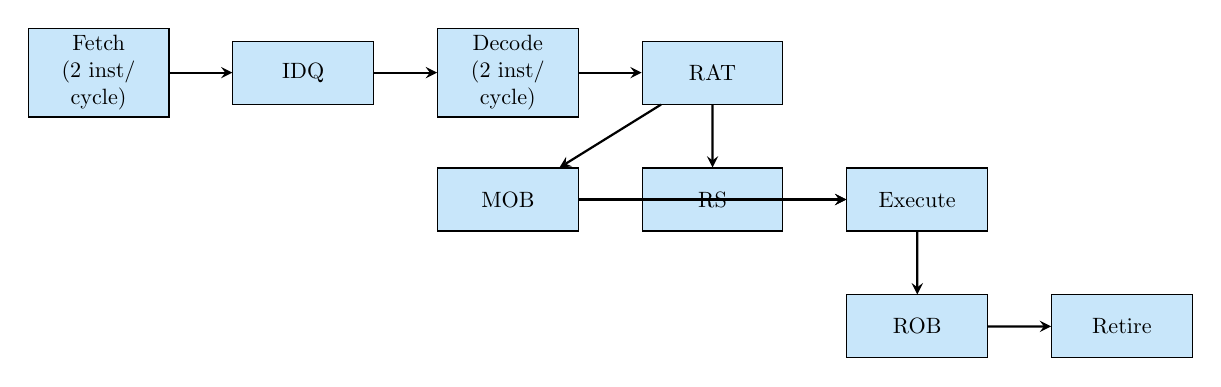
\begin{tikzpicture}[scale=0.8, transform shape]
    % Define styles
    \tikzstyle{block} = [rectangle, draw, fill=lightblue, 
                          text width=2cm, text centered, 
                          minimum height=1cm]
    \tikzstyle{arrow} = [thick,->,>=stealth]
    
    % Create blocks
    \node[block] (fetch) {Fetch\\(2~inst\slash cycle)};
    \node[block, right=of fetch] (idq) {IDQ};
    \node[block, right=of idq] (decode) {Decode\\(2~inst\slash cycle)};
    \node[block, right=of decode] (rat) {RAT};
    
    \node[block, below=of rat] (rs) {RS};
    \node[block, right=of rs] (exec) {Execute};
    \node[block, left=of rs] (mob) {MOB};
    
    \node[block, below=of exec] (rob) {ROB};
    \node[block, right=of rob] (retire) {Retire};
    
    % Draw arrows
    \draw[arrow] (fetch) -- (idq);
    \draw[arrow] (idq) -- (decode);
    \draw[arrow] (decode) -- (rat);
    \draw[arrow] (rat) -- (rs);
    \draw[arrow] (rat) -- (mob);
    \draw[arrow] (rs) -- (exec);
    \draw[arrow] (mob) -- (exec);
    \draw[arrow] (exec) -- (rob);
    \draw[arrow] (rob) -- (retire);
\end{tikzpicture}
\end{figure}
\end{frame}

\begin{frame}{Execution Timeline - Second Loop Iteration}
\begin{block}{Question}
Show the system state when completing the fetch of instruction L1 for the second time.
\end{block}

\begin{itemize}
    \item Track instruction flow through pipeline stages
    \item Monitor reservation stations and ROB entries
    \item Identify dependencies and hazards
    \item Calculate execution cycles
\end{itemize}
\end{frame}

% Initial state
\begin{frame}{OOOE: Initial State}
\OOODiagramKV[
    showcode=1,
]
\end{frame}

% Cycle 1
\begin{frame}{OOOE: Cycle 1}
\OOODiagramKV[
    idq1=\newentryb{SUB R1,R1,R1},
    idq2=\newentrya{ADDI R10,R0,100},
    showcode=1,
    highlight1=1,
    highlight2=2,
]
\end{frame}

% Cycle 2 - Multiple slides to show progression
\begin{frame}{OOOE: Cycle 2, Instruction Decode}
\OOODiagramKV[
    R1=\newentryb{RB1},
    R10=\newentrya{RB0},
    idq1=\newentryb{\sout{SUB R1,R1,R1}},
    idq2=\newentrya{\sout{ADDI R10,R0,100}},
    rs1=\newentrya{RB0$\leftarrow$R0+100},
    rs2=\newentryb{RB1$\leftarrow$R1-R1},
    robleft0={RB0},
    rob01=\newentrya{ADDI R10,R0,100},
    rob02=\newentrya{INV},
    robleft1={RB1},
    rob11=\newentryb{SUB R1,R1,R1},
    rob12=\newentryb{INV},
    showcode=1,
]
\end{frame}

\begin{frame}{OOOE: Cycle 2, Instruction Fetch}
\OOODiagramKV[
    R1=\oldentry{RB1},
    R10=\oldentry{RB0},
    idq1=\newentryb{LW R5,100(R4)},
    idq2=\newentrya{ADDI R4,R0,20},
    rs1=\oldentry{RB0$\leftarrow$R0+100},
    rs2=\oldentry{RB1$\leftarrow$R1-R1},
    robleft0=\oldentry{RB0},
    rob01=\oldentry{ADDI R10,R0,100},
    rob02=\oldentry{INV},
    robleft1=\oldentry{RB1},
    rob11=\oldentry{SUB R1,R1,R1},
    rob12=\oldentry{INV},
    showcode=1,
    highlight1=3,
    highlight2=4,
]
\end{frame}

% Cycle 3 - Multiple slides
\begin{frame}{OOOE: Cycle 3, Execution Starts}
\OOODiagramKV[
    R1=\oldentry{RB1},
    R10=\oldentry{RB0},
    idq1=\oldentry{LW R5,100(R4)},
    idq2=\oldentry{ADDI R4,R0,20},
    rs1=\srcentrya{\sout{RB0$\leftarrow$R0+100}},
    rs2=\srcentryb{\sout{RB1$\leftarrow$R1-R1}},
    robleft0=\oldentry{RB0},
    rob01=\oldentry{ADDI R10,R0,100},
    rob02=\oldentry{INV},
    robleft1=\oldentry{RB1},
    rob11=\oldentry{SUB R1,R1,R1},
    rob12=\oldentry{INV},
    exec1=\newentrya{RB0$\leftarrow$R0+100},
    exec2=\newentryb{RB1$\leftarrow$R1-R1},
    showcode=1,
]
\end{frame}

\begin{frame}{OOOE: Cycle 3, Instruction Decode}
\OOODiagramKV[
    R1=\oldentry{RB1}, R10=\oldentry{RB0},
    R4=\newentrya{RB2}, R5=\newentryb{RB3},
    idq1=\srcentryb{\sout{LW R5,100(R4)}},
    idq2=\srcentrya{\sout{ADDI R4,R0,20}},
    rs1=\oldentry{\sout{RB0$\leftarrow$R0+100}},
    rs2=\oldentry{\sout{RB1$\leftarrow$R1-R1}},
    rs3=\newentrya{RB2$\leftarrow$R0+20},
    robleft0=\oldentry{RB0},
    rob01=\oldentry{ADDI R10,R0,100},
    rob02=\oldentry{INV},
    robleft1=\oldentry{RB1},
    rob11=\oldentry{SUB R1,R1,R1},
    rob12=\oldentry{INV},
    robleft2={RB2},
    rob21=\newentrya{ADDI R4,R0,20},
    rob22=\newentrya{INV},
    robleft3={RB3},
    rob31=\newentryb{LW R5,100(R4)},
    rob32=\newentryb{INV},
    mob1=\newentryb{RB3$\leftarrow$LD(RB2+100)},
    exec1=\oldentry{RB0$\leftarrow$R0+100},
    exec2=\oldentry{RB1$\leftarrow$R1-R1},
    showcode=1,
]
\end{frame}

\begin{frame}{OOOE: Cycle 3, Instruction Fetch}
\OOODiagramKV[
    R1=\oldentry{RB1}, R10=\oldentry{RB0},
    R4=\oldentry{RB2}, R5=\oldentry{RB3},
    idq1=\newentryb{ADDI R5, R3, 2},
    idq2=\newentrya{ADDI R3, R2, 2},
    rs1=\oldentry{\sout{RB0$\leftarrow$R0+100}},
    rs2=\oldentry{\sout{RB1$\leftarrow$R1-R1}},
    rs3=\oldentry{RB2$\leftarrow$R0+20},
    robleft0=\oldentry{RB0},
    rob01=\oldentry{ADDI R10,R0,100},
    rob02=\oldentry{INV},
    robleft1=\oldentry{RB1},
    rob11=\oldentry{SUB R1,R1,R1},
    rob12=\oldentry{INV},
    robleft2=\oldentry{RB2},
    rob21=\oldentry{ADDI R4,R0,20},
    rob22=\oldentry{INV},
    robleft3=\oldentry{RB3},
    rob31=\oldentry{LW R5,100(R4)},
    rob32=\oldentry{INV},
    mob1=\oldentry{RB3$\leftarrow$LD(RB2+100)},
    exec1=\oldentry{RB0$\leftarrow$R0+100},
    exec2=\oldentry{RB1$\leftarrow$R1-R1},
    showcode=1,
    highlight1=5,
    highlight2=6,
]
\end{frame}

% Cycle 4 - Multiple slides
\begin{frame}{OOOE: Cycle 4, Execution Completed}
\OOODiagramKV[
    R1=\oldentry{RB1}, R10=\oldentry{RB0},
    R4=\oldentry{RB2}, R5=\oldentry{RB3},
    idq1=\oldentry{ADDI R5, R3, 2},
    idq2=\oldentry{ADDI R3, R2, 2},
    rs3=\oldentry{RB2$\leftarrow$R0+20},
    robleft0=\oldentry{RB0},
    rob01=\oldentry{ADDI R10,R0,100},
    rob02=\newentrya{OK},
    robleft1=\oldentry{RB1},
    rob11=\oldentry{SUB R1,R1,R1},
    rob12=\newentryb{OK},
    robleft2=\oldentry{RB2},
    rob21=\oldentry{ADDI R4,R0,20},
    rob22=\oldentry{INV},
    robleft3=\oldentry{RB3},
    rob31=\oldentry{LW R5,100(R4)},
    rob32=\oldentry{INV},
    mob1=\oldentry{RB3$\leftarrow$LD(RB2+100)},
    exec1=\newentrya{\sout{RB0$\leftarrow$R0+100}},
    exec2=\newentryb{\sout{RB1$\leftarrow$R1-R1}},
    showcode=1,
]
\end{frame}

\begin{frame}{OOOE: Cycle 4, Execution Starts}
\OOODiagramKV[
    R1=\oldentry{RB1}, R10=\oldentry{RB0},
    R4=\oldentry{RB2}, R5=\oldentry{RB3},
    idq1=\oldentry{ADDI R5, R3, 2},
    idq2=\oldentry{ADDI R3, R2, 2},
    rs3=\srcentrya{\sout{RB2$\leftarrow$R0+20}},
    robleft0=\oldentry{RB0},
    rob01=\oldentry{ADDI R10,R0,100},
    rob02=\oldentry{OK},
    robleft1=\oldentry{RB1},
    rob11=\oldentry{SUB R1,R1,R1},
    rob12=\oldentry{OK},
    robleft2=\oldentry{RB2},
    rob21=\oldentry{ADDI R4,R0,20},
    rob22=\oldentry{INV},
    robleft3=\oldentry{RB3},
    rob31=\oldentry{LW R5,100(R4)},
    rob32=\oldentry{INV},
    mob1=\oldentry{RB3$\leftarrow$LD(RB2+100)},
    exec1=\newentrya{RB2$\leftarrow$R0+20},
    showcode=1,
]
\end{frame}

\begin{frame}{OOOE: Cycle 4, Stall on Dependencies}
\OOODiagramKV[
    R1=\oldentry{RB1}, R10=\oldentry{RB0},
    R4=\oldentry{RB2}, R5=\oldentry{RB3},
    idq1=\oldentry{ADDI R5, R3, 2},
    idq2=\oldentry{ADDI R3, R2, 2},
    rs3=\oldentry{\sout{RB2$\leftarrow$R0+20}},
    robleft0=\oldentry{RB0},
    rob01=\oldentry{ADDI R10,R0,100},
    rob02=\oldentry{OK},
    robleft1=\oldentry{RB1},
    rob11=\oldentry{SUB R1,R1,R1},
    rob12=\oldentry{OK},
    robleft2={RB2},
    rob21=\oldentry{ADDI R4,R0,20},
    rob22=\srcentryb{INV},
    robleft3=\oldentry{RB3},
    rob31=\oldentry{LW R5,100(R4)},
    rob32=\oldentry{INV},
    mob1=\newentryb{RB3$\leftarrow$LD(RB2+100)},
    exec1=\srcentryb{RB2$\leftarrow$R0+20},
    showcode=1,
]
\end{frame}

\begin{frame}{OOOE: Cycle 4, Decode}
\OOODiagramKV[
    R1=\oldentry{RB1}, R10=\oldentry{RB0},
    R3=\newentrya{RB4},
    R4=\oldentry{RB2}, R5=\newentryb{RB5},
    idq1=\newentryb{\sout{ADDI R5, R3, 2}},
    idq2=\newentrya{\sout{ADDI R3, R2, 2}},
    rs1=\newentrya{RB4$\leftarrow$R2+2},
    rs2=\newentryb{RB5$\leftarrow$RB4+2},
    rs3=\oldentry{\sout{RB2$\leftarrow$R0+20}},
    robleft0=\oldentry{RB0},
    rob01=\oldentry{ADDI R10,R0,100},
    rob02=\oldentry{OK},
    robleft1=\oldentry{RB1},
    rob11=\oldentry{SUB R1,R1,R1},
    rob12=\oldentry{OK},
    robleft2=\oldentry{RB2},
    rob21=\oldentry{ADDI R4,R0,20},
    rob22=\oldentry{INV},
    robleft3=\oldentry{RB3},
    rob31=\oldentry{LW R5,100(R4)},
    rob32=\oldentry{INV},
    robleft4={RB4},
    rob41=\newentrya{ADDI R3,R2,2},
    rob42=\newentrya{INV},
    robleft5={RB5},
    rob51=\newentryb{ADDI R5,R3,2},
    rob52=\newentryb{INV},
    mob1=\oldentry{RB3$\leftarrow$LD(RB2+100)},
    exec1=\oldentry{RB2$\leftarrow$R0+20},
    showcode=1,
]
\end{frame}

\begin{frame}{OOOE: Cycle 4, Fetch}
\OOODiagramKV[
    R1=\oldentry{RB1}, R10=\oldentry{RB0},
    R3=\oldentry{RB4},
    R4=\oldentry{RB2}, R5=\oldentry{RB5},
    idq1=\newentryb{ADD R7, R5, R0},
    idq2=\newentrya{ADDI R6, R0, 6},
    rs1=\oldentry{RB4$\leftarrow$R2+2},
    rs2=\oldentry{RB5$\leftarrow$RB4+2},
    rs3=\oldentry{\sout{RB2$\leftarrow$R0+20}},
    robleft0=\oldentry{RB0},
    rob01=\oldentry{ADDI R10,R0,100},
    rob02=\oldentry{OK},
    robleft1=\oldentry{RB1},
    rob11=\oldentry{SUB R1,R1,R1},
    rob12=\oldentry{OK},
    robleft2=\oldentry{RB2},
    rob21=\oldentry{ADDI R4,R0,20},
    rob22=\oldentry{INV},
    robleft3=\oldentry{RB3},
    rob31=\oldentry{LW R5,100(R4)},
    rob32=\oldentry{INV},
    robleft4=\oldentry{RB4},
    rob41=\oldentry{ADDI R3,R2,2},
    rob42=\oldentry{INV},
    robleft5=\oldentry{RB5},
    rob51=\oldentry{ADDI R5,R3,2},
    rob52=\oldentry{INV},
    mob1=\oldentry{RB3$\leftarrow$LD(RB2+100)},
    exec1=\oldentry{RB2$\leftarrow$R0+20},
    showcode=1,
    highlight1=7,
    highlight2=8,
]
\end{frame}

% Continue with remaining cycles following the same pattern...
% (I'll continue with a few more key cycles)

\begin{frame}{OOOE: Cycle 5, Retire}
\OOODiagramKV[
    R1=\newentryb{\sout{RB1}}, R10=\newentrya{\sout{RB0}},
    R3=\oldentry{RB4},
    R4=\oldentry{RB2}, R5=\oldentry{RB5},
    idq1=\oldentry{ADD R7, R5, R0},
    idq2=\oldentry{ADDI R6, R0, 6},
    rs1=\oldentry{RB4$\leftarrow$R2+2},
    rs2=\oldentry{RB5$\leftarrow$RB4+2},
    robleft0={\sout{RB0}},
    rob01=\srcentrya{\sout{ADDI R10,R0,100}},
    rob02=\srcentrya{OK},
    robleft1={\sout{RB1}},
    rob11=\srcentryb{\sout{SUB R1,R1,R1}},
    rob12=\srcentryb{OK},
    robleft2=\oldentry{RB2},
    rob21=\oldentry{ADDI R4,R0,20},
    rob22=\oldentry{INV},
    robleft3=\oldentry{RB3},
    rob31=\oldentry{LW R5,100(R4)},
    rob32=\oldentry{INV},
    robleft4=\oldentry{RB4},
    rob41=\oldentry{ADDI R3,R2,2},
    rob42=\oldentry{INV},
    robleft5=\oldentry{RB5},
    rob51=\oldentry{ADDI R5,R3,2},
    rob52=\oldentry{INV},
    mob1=\oldentry{RB3$\leftarrow$LD(RB2+100)},
    exec1=\oldentry{RB2$\leftarrow$R0+20},
    ret1=\newentrya{R10$\leftarrow$RB0},
    ret2=\newentryb{R1$\leftarrow$RB1},
    showcode=1,
]
\end{frame}

% Cycle 6 - Multiple slides showing progression
\begin{frame}{OOOE: Cycle 6, Retire}
\OOODiagramKV[
    R3=\oldentry{RB4},
    R4=\srcentrya{\sout{RB2}}, R5=\oldentry{RB5},
    R6=\oldentry{RB6},
    R7=\oldentry{RB7},
    idq1=\oldentry{ADDI R9, R0, 9},
    idq2=\oldentry{ADDI R8, R0, 8},
    rs2=\oldentry{RB5$\leftarrow$RB4+2},
    rs3=\oldentry{RB6$\leftarrow$R0+6},
    rs5=\oldentry{RB7$\leftarrow$RB5+R0},
    robleft2={\sout{RB2}},
    rob21=\srcentrya{\sout{ADDI R4,R0,20}},
    rob22=\srcentrya{OK},
    robleft3=\oldentry{RB3},
    rob31=\oldentry{LW R5,100(R4)},
    rob32=\oldentry{INV},
    robleft4=\oldentry{RB4},
    rob41=\oldentry{ADDI R3,R2,2},
    rob42=\oldentry{INV},
    robleft5=\oldentry{RB5},
    rob51=\oldentry{ADDI R5,R3,2},
    rob52=\oldentry{INV},
    robleft6=\oldentry{RB6},
    rob61=\oldentry{ADDI R6,R0,6},
    rob62=\oldentry{INV},
    robleft7=\oldentry{RB7},
    rob71=\oldentry{ADDI R7,R5,R0},
    rob72=\oldentry{INV},
    mob1=\oldentry{RB3$\leftarrow$LD(RB2+100)},
    ret1=\newentrya{R4$\leftarrow$RB2},
    exec1=\oldentry{RB3$\leftarrow$RB2+100},
    exec2=\oldentry{RB4$\leftarrow$R2+2},
    showcode=1,
]
\end{frame}

\begin{frame}{OOOE: Cycle 6, Execution Completed / Load Issued}
\OOODiagramKV[
    R3=\oldentry{RB4},
    R5=\oldentry{RB5},
    R6=\oldentry{RB6},
    R7=\oldentry{RB7},
    idq1=\oldentry{ADDI R9, R0, 9},
    idq2=\oldentry{ADDI R8, R0, 8},
    rs2=\oldentry{RB5$\leftarrow$RB4+2},
    rs3=\oldentry{RB6$\leftarrow$R0+6},
    rs5=\oldentry{RB7$\leftarrow$RB5+R0},
    robleft3=\oldentry{RB3},
    rob31=\oldentry{LW R5,100(R4)},
    rob32=\oldentry{INV},
    robleft4=\oldentry{RB4},
    rob41=\oldentry{ADDI R3,R2,2},
    rob42=\newentryb{OK},
    robleft5=\oldentry{RB5},
    rob51=\oldentry{ADDI R5,R3,2},
    rob52=\oldentry{INV},
    robleft6=\oldentry{RB6},
    rob61=\oldentry{ADDI R6,R0,6},
    rob62=\oldentry{INV},
    robleft7=\oldentry{RB7},
    rob71=\oldentry{ADDI R7,R5,R0},
    rob72=\oldentry{INV},
    mob1=\newentrya{RB3$\leftarrow$LD(RB2+100)},
    mobmark1=\newentrya{(1)},
    ret1=\oldentry{R4$\leftarrow$RB2},
    exec1=\srcentrya{RB3$\leftarrow$RB2+100},
    exec2=\srcentryb{RB4$\leftarrow$R2+2},
    showcode=1,
]
\end{frame}

\begin{frame}{OOOE: Cycle 6, Execution Starts}
\OOODiagramKV[
    R3=\oldentry{RB4},
    R5=\oldentry{RB5},
    R6=\oldentry{RB6},
    R7=\oldentry{RB7},
    idq1=\oldentry{ADDI R9, R0, 9},
    idq2=\oldentry{ADDI R8, R0, 8},
    rs2=\srcentrya{\sout{RB5$\leftarrow$RB4+2}},
    rs3=\srcentryb{\sout{RB6$\leftarrow$R0+6}},
    rs5=\oldentry{RB7$\leftarrow$RB5+R0},
    robleft3=\oldentry{RB3},
    rob31=\oldentry{LW R5,100(R4)},
    rob32=\oldentry{INV},
    robleft4=\oldentry{RB4},
    rob41=\oldentry{ADDI R3,R2,2},
    rob42=\oldentry{OK},
    robleft5=\oldentry{RB5},
    rob51=\oldentry{ADDI R5,R3,2},
    rob52=\oldentry{INV},
    robleft6=\oldentry{RB6},
    rob61=\oldentry{ADDI R6,R0,6},
    rob62=\oldentry{INV},
    robleft7=\oldentry{RB7},
    rob71=\oldentry{ADDI R7,R5,R0},
    rob72=\oldentry{INV},
    mob1=\oldentry{RB3$\leftarrow$LD(RB2+100)},
    mobmark1=\oldentry{(1)},
    exec1=\newentrya{RB5$\leftarrow$RB4+2},
    exec2=\newentryb{RB6$\leftarrow$R0+6},
    showcode=1,
]
\end{frame}

\begin{frame}{OOOE: Cycle 6, Instruction Decode}
\OOODiagramKV[
    R3=\oldentry{RB4},
    R5=\oldentry{RB5},
    R6=\oldentry{RB6},
    R7=\oldentry{RB7},
    R8=\newentryb{RB8},
    R9=\newentrya{RB0},
    idq1=\srcentrya{\sout{ADDI R9, R0, 9}},
    idq2=\srcentryb{\sout{ADDI R8, R0, 8}},
    rs1=\newentrya{RB8$\leftarrow$R0+8},
    rs2=\oldentry{\sout{RB5$\leftarrow$RB4+2}},
    rs3=\oldentry{\sout{RB6$\leftarrow$R0+6}},
    rs4=\newentryb{RB0$\leftarrow$R0+9},
    rs5=\oldentry{RB7$\leftarrow$RB5+R0},
    robleft0={RB0},
    rob01=\newentrya{ADDI R9,R0,9},
    rob02=\newentrya{INV},
    robleft3=\oldentry{RB3},
    rob31=\oldentry{LW R5,100(R4)},
    rob32=\oldentry{INV},
    robleft4=\oldentry{RB4},
    rob41=\oldentry{ADDI R3,R2,2},
    rob42=\oldentry{OK},
    robleft5=\oldentry{RB5},
    rob51=\oldentry{ADDI R5,R3,2},
    rob52=\oldentry{INV},
    robleft6=\oldentry{RB6},
    rob61=\oldentry{ADDI R6,R0,6},
    rob62=\oldentry{INV},
    robleft7=\oldentry{RB7},
    rob71=\oldentry{ADDI R7,R5,R0},
    rob72=\oldentry{INV},
    robleft8={RB8},
    rob81=\newentryb{ADDI R8,R0,8},
    rob82=\newentryb{INV},
    mob1=\oldentry{RB3$\leftarrow$LD(RB2+100)},
    mobmark1=\oldentry{(1)},
    exec1=\oldentry{RB5$\leftarrow$RB4+2},
    exec2=\oldentry{RB6$\leftarrow$R0+6},
    showcode=1,
    highlight1=9,
    highlight2=10,
]
\end{frame}

\begin{frame}{OOOE: Cycle 6, Instruction Fetch}
\OOODiagramKV[
    R3=\oldentry{RB4},
    R5=\oldentry{RB5},
    R6=\oldentry{RB6},
    R7=\oldentry{RB7},
    R8=\oldentry{RB8},
    R9=\oldentry{RB0},
    idq1=\newentryb{BNE R1, R10, L1},
    idq2=\newentrya{ADDI R1,R1,1},
    rs1=\oldentry{RB8$\leftarrow$R0+8},
    rs2=\oldentry{\sout{RB5$\leftarrow$RB4+2}},
    rs3=\oldentry{\sout{RB6$\leftarrow$R0+6}},
    rs4=\oldentry{RB0$\leftarrow$R0+9},
    rs5=\oldentry{RB7$\leftarrow$RB5+R0},
    robleft0=\oldentry{RB0},
    rob01=\oldentry{ADDI R9,R0,9},
    rob02=\oldentry{INV},
    robleft3=\oldentry{RB3},
    rob31=\oldentry{LW R5,100(R4)},
    rob32=\oldentry{INV},
    robleft4=\oldentry{RB4},
    rob41=\oldentry{ADDI R3,R2,2},
    rob42=\oldentry{OK},
    robleft5=\oldentry{RB5},
    rob51=\oldentry{ADDI R5,R3,2},
    rob52=\oldentry{INV},
    robleft6=\oldentry{RB6},
    rob61=\oldentry{ADDI R6,R0,6},
    rob62=\oldentry{INV},
    robleft7=\oldentry{RB7},
    rob71=\oldentry{ADDI R7,R5,R0},
    rob72=\oldentry{INV},
    robleft8=\oldentry{RB8},
    rob81=\oldentry{ADDI R8,R0,8},
    rob82=\oldentry{INV},
    mob1=\oldentry{RB3$\leftarrow$LD(RB2+100)},
    mobmark1=\oldentry{(1)},
    exec1=\oldentry{RB5$\leftarrow$RB4+2},
    exec2=\oldentry{RB6$\leftarrow$R0+6},
    showcode=1,
    highlight1=11,
    highlight2=12,
]
\end{frame}

% Cycle 7 - Second iteration begins
\begin{frame}{OOOE: Cycle 7, Retire}
\OOODiagramKV[
    R3=\newentrya{\sout{RB4}},
    R5=\oldentry{RB5},
    R6=\oldentry{RB6},
    R7=\oldentry{RB7},
    R8=\oldentry{RB8},
    R9=\oldentry{RB0},
    idq1=\oldentry{BNE R1, R10, L1},
    idq2=\oldentry{ADDI R1,R1,1},
    rs1=\oldentry{RB8$\leftarrow$R0+8},
    rs4=\oldentry{RB0$\leftarrow$R0+9},
    rs5=\oldentry{RB7$\leftarrow$RB5+R0},
    robleft0=\oldentry{RB0},
    rob01=\oldentry{ADDI R9,R0,9},
    rob02=\oldentry{INV},
    robleft3=\oldentry{RB3},
    rob31=\oldentry{LW R5,100(R4)},
    rob32=\oldentry{INV},
    robleft4={\sout{RB4}},
    rob41=\newentrya{\sout{ADDI R3,R2,2}},
    rob42=\srcentrya{OK},
    robleft5=\oldentry{RB5},
    rob51=\oldentry{ADDI R5,R3,2},
    rob52=\oldentry{INV},
    robleft6=\oldentry{RB6},
    rob61=\oldentry{ADDI R6,R0,6},
    rob62=\oldentry{INV},
    robleft7=\oldentry{RB7},
    rob71=\oldentry{ADDI R7,R5,R0},
    rob72=\oldentry{INV},
    robleft8=\oldentry{RB8},
    rob81=\oldentry{ADDI R8,R0,8},
    rob82=\oldentry{INV},
    mob1=\oldentry{RB3$\leftarrow$LD(RB2+100)},
    mobmark1=\oldentry{(1)},
    ret1=\newentrya{R3$\leftarrow$RB4},
    exec1=\oldentry{RB5$\leftarrow$RB4+2},
    exec2=\oldentry{RB6$\leftarrow$R0+6},
    showcode=1,
]
\end{frame}

\begin{frame}{OOOE: Cycle 7, Execution Completed}
\OOODiagramKV[
    R3=\oldentry{\sout{RB4}},
    R5=\oldentry{RB5},
    R6=\oldentry{RB6},
    R7=\oldentry{RB7},
    R8=\oldentry{RB8},
    R9=\oldentry{RB0},
    idq1=\oldentry{BNE R1, R10, L1},
    idq2=\oldentry{ADDI R1,R1,1},
    rs1=\oldentry{RB8$\leftarrow$R0+8},
    rs4=\oldentry{RB0$\leftarrow$R0+9},
    rs5=\oldentry{RB7$\leftarrow$RB5+R0},
    robleft0=\oldentry{RB0},
    rob01=\oldentry{ADDI R9,R0,9},
    rob02=\oldentry{INV},
    robleft3=\oldentry{RB3},
    rob31=\oldentry{LW R5,100(R4)},
    rob32=\oldentry{INV},
    robleft5=\oldentry{RB5},
    rob51=\oldentry{ADDI R5,R3,2},
    rob52=\newentrya{OK},
    robleft6=\oldentry{RB6},
    rob61=\oldentry{ADDI R6,R0,6},
    rob62=\newentryb{OK},
    robleft7=\oldentry{RB7},
    rob71=\oldentry{ADDI R7,R5,R0},
    rob72=\oldentry{INV},
    robleft8=\oldentry{RB8},
    rob81=\oldentry{ADDI R8,R0,8},
    rob82=\oldentry{INV},
    mob1=\oldentry{RB3$\leftarrow$LD(RB2+100)},
    mobmark1=\newentrya{(2)},
    ret1=\oldentry{R3$\leftarrow$RB4},
    exec1=\srcentrya{RB5$\leftarrow$RB4+2},
    exec2=\srcentryb{RB6$\leftarrow$R0+6},
    showcode=1,
]
\end{frame}

\begin{frame}{OOOE: Cycle 7, Execution Starts}
\OOODiagramKV[
    R3=\oldentry{\sout{RB4}},
    R5=\oldentry{RB5},
    R6=\oldentry{RB6},
    R7=\oldentry{RB7},
    R8=\oldentry{RB8},
    R9=\oldentry{RB0},
    idq1=\oldentry{BNE R1, R10, L1},
    idq2=\oldentry{ADDI R1,R1,1},
    rs1=\srcentryb{\sout{RB8$\leftarrow$R0+8}},
    rs4=\oldentry{RB0$\leftarrow$R0+9},
    rs5=\srcentrya{\sout{RB7$\leftarrow$RB5+R0}},
    robleft0=\oldentry{RB0},
    rob01=\oldentry{ADDI R9,R0,9},
    rob02=\oldentry{INV},
    robleft3=\oldentry{RB3},
    rob31=\oldentry{LW R5,100(R4)},
    rob32=\oldentry{INV},
    robleft5=\oldentry{RB5},
    rob51=\oldentry{ADDI R5,R3,2},
    rob52=\oldentry{OK},
    robleft6=\oldentry{RB6},
    rob61=\oldentry{ADDI R6,R0,6},
    rob62=\oldentry{OK},
    robleft7=\oldentry{RB7},
    rob71=\oldentry{ADDI R7,R5,R0},
    rob72=\oldentry{INV},
    robleft8=\oldentry{RB8},
    rob81=\oldentry{ADDI R8,R0,8},
    rob82=\oldentry{INV},
    mob1=\oldentry{RB3$\leftarrow$LD(RB2+100)},
    mobmark1=\oldentry{(2)},
    exec1=\newentrya{RB7$\leftarrow$RB5+R0},
    exec2=\newentryb{RB8$\leftarrow$R0+8},
    showcode=1,
]
\end{frame}

\begin{frame}{OOOE: Cycle 7, Instruction Decode}
\OOODiagramKV[
    R1=\newentrya{RB1},
    R3=\oldentry{\sout{RB4}},
    R5=\oldentry{RB5},
    R6=\oldentry{RB6},
    R7=\oldentry{RB7},
    R8=\oldentry{RB8},
    R9=\oldentry{RB0},
    idq1=\srcentryb{\sout{BNE R1, R10, L1}},
    idq2=\srcentrya{\sout{ADDI R1,R1,1}},
    rs1=\oldentry{\sout{RB8$\leftarrow$R0+8}},
    rs2=\newentrya{RB1$\leftarrow$R1+1},
    rs3=\newentryb{RB2$\leftarrow$RB1-R10},
    rs4=\oldentry{RB0$\leftarrow$R0+9},
    rs5=\oldentry{\sout{RB7$\leftarrow$RB5+R0}},
    robleft0=\oldentry{RB0},
    rob01=\oldentry{ADDI R9,R0,9},
    rob02=\oldentry{INV},
    robleft1={RB1},
    rob11=\newentrya{ADDI R1,R1,1},
    rob12=\newentrya{INV},
    robleft2={RB2},
    rob21=\newentryb{BNE R1,R10,L1},
    rob22=\newentryb{INV},
    robleft3=\oldentry{RB3},
    rob31=\oldentry{LW R5,100(R4)},
    rob32=\oldentry{INV},
    robleft5=\oldentry{RB5},
    rob51=\oldentry{ADDI R5,R3,2},
    rob52=\oldentry{OK},
    robleft6=\oldentry{RB6},
    rob61=\oldentry{ADDI R6,R0,6},
    rob62=\oldentry{OK},
    robleft7=\oldentry{RB7},
    rob71=\oldentry{ADDI R7,R5,R0},
    rob72=\oldentry{INV},
    robleft8=\oldentry{RB8},
    rob81=\oldentry{ADDI R8,R0,8},
    rob82=\oldentry{INV},
    mob1=\oldentry{RB3$\leftarrow$LD(RB2+100)},
    mobmark1=\oldentry{(2)},
    exec1=\oldentry{RB7$\leftarrow$RB5+R0},
    exec2=\oldentry{RB8$\leftarrow$R0+8},
    showcode=1,
]
\end{frame}

\begin{frame}{OOOE: Cycle 7, Second Iteration Fetch}
\OOODiagramKV[
    R1=\newentrya{RB1},
    R3=\oldentry{\sout{RB4}},
    R5=\oldentry{RB5},
    R6=\oldentry{RB6},
    R7=\oldentry{RB7},
    R8=\oldentry{RB8},
    R9=\oldentry{RB0},
    idq1=\newentryb{LW R5,100(R4)},
    idq2=\newentrya{ADDI R4,R0,20},
    rs1=\srcentryb{\sout{RB8$\leftarrow$R0+8}},
    rs2=\newentrya{RB1$\leftarrow$R1+1},
    rs3=\newentryb{RB2$\leftarrow$RB1-R10},
    rs4=\oldentry{RB0$\leftarrow$R0+9},
    rs5=\srcentrya{\sout{RB7$\leftarrow$RB5+R0}},
    robleft0=\oldentry{RB0},
    rob01=\oldentry{ADDI R9,R0,9},
    rob02=\oldentry{INV},
    robleft1={RB1},
    rob11=\newentrya{ADDI R1,R1,1},
    rob12=\newentrya{INV},
    robleft2={RB2},
    rob21=\newentryb{BNE R1,R10,L1},
    rob22=\newentryb{INV},
    robleft3=\oldentry{RB3},
    rob31=\oldentry{LW R5,100(R4)},
    rob32=\oldentry{INV},
    robleft4={\sout{RB4}},
    rob41=\oldentry{\sout{ADDI R3,R2,2}},
    rob42=\oldentry{OK},
    robleft5=\oldentry{RB5},
    rob51=\oldentry{ADDI R5,R3,2},
    rob52=\newentrya{OK},
    robleft6=\oldentry{RB6},
    rob61=\oldentry{ADDI R6,R0,6},
    rob62=\newentryb{OK},
    robleft7=\oldentry{RB7},
    rob71=\oldentry{ADDI R7,R5,R0},
    rob72=\oldentry{INV},
    robleft8=\oldentry{RB8},
    rob81=\oldentry{ADDI R8,R0,8},
    rob82=\oldentry{INV},
    mob1=\oldentry{RB3$\leftarrow$LD(RB2+100)},
    mobmark1=\newentrya{(2)},
    ret1=\newentrya{R3$\leftarrow$RB4},
    exec1=\newentrya{RB7$\leftarrow$RB5+R0},
    exec2=\newentryb{RB8$\leftarrow$R0+8},
    showcode=1,
    highlight1=3,
    highlight2=4,
]
\end{frame}

\section{Performance Analysis}

\begin{frame}{Key Execution Cycles}
\begin{table}
\centering
\begin{tabular}{|c|l|l|}
\hline
\textbf{Cycle} & \textbf{Operations} & \textbf{Notes} \\
\hline
1 & Fetch first 2 instructions & ADDI R10, SUB R1 \\
\hline
2 & Decode, Fetch next 2 & ADDI R4, LW R5 \\
\hline
3 & Issue to RS/MOB & Load enters MOB \\
\hline
4-6 & Execute ALU ops & Load in progress \\
\hline
7 & Second iteration fetch & RAW dependency \\
\hline
\end{tabular}
\end{table}

\begin{alertblock}{Critical Path}
The load instruction creates a 5-cycle latency that affects dependent instructions.
\end{alertblock}
\end{frame}

\begin{frame}{CPI Calculation}
\begin{block}{Performance Metrics}
\begin{itemize}
    \item Loop contains 10 instructions
    \item Executes 100 iterations
    \item From first LW fetch (cycle 2) to second LW fetch (cycle 7): 5 cycles
    \item No delays from memory reads after first iteration
    \item Structural hazard doesn't cause delays (only 1 instruction in EXE at times)
\end{itemize}
\end{block}

\begin{tcolorbox}[colback=highlightyellow,colframe=darkblue]
\textbf{Result:} CPI $\approx$ 0.5
\begin{itemize}
    \item System can sustain 2 instructions per cycle
    \item OOO execution hides latencies effectively
\end{itemize}
\end{tcolorbox}
\end{frame}

\section{Compiler Optimization}

\begin{frame}[fragile]{Compiler Optimization}
\begin{columns}
\column{0.45\textwidth}
\textbf{Original Code:}
\begin{lstlisting}[basicstyle=\ttfamily\tiny]
R0 = 0
R1 = 0
L1: R4 = 20
    R5 = load 100(R4)
    R3 = R2+2
    R5 = R3 + 2
    R6 = 6
    R7 = R5
    R8 = 8
    R9 = 9
    R1 = R1 + 1
    IF (R1 < 100) goto L1
L2: R4 = 23
\end{lstlisting}

\column{0.45\textwidth}
\textbf{Optimized Code:}
\begin{lstlisting}[basicstyle=\ttfamily\tiny]
R0 = 0
R1 = 0
R4 = 20
R6 = 6
R8 = 8
R9 = 9
L1: R5 = load 100(R4)
    R3 = R2+2
    R5 = R3 + 2
    R1 = R1 + 1
    IF (R1 < 100) goto L1
R7 = R5
L2: R4 = 23
\end{lstlisting}
\end{columns}

\begin{block}{Optimization: Loop Invariant Code Motion}
Move constant assignments outside the loop!
\end{block}
\end{frame}

\begin{frame}{Impact of Optimization}
\begin{columns}[t]
\column{0.48\textwidth}
\begin{block}{Analysis}
\begin{itemize}
    \item \textbf{Before:} 10 instructions in loop
    \item \textbf{After:} 5 instructions in loop
    \item \textbf{BUT:} Load operation still takes 5 cycles
    \item Load operations cannot execute in parallel
\end{itemize}
\end{block}

\column{0.48\textwidth}
\begin{alertblock}{Performance Result}
\begin{itemize}
    \item CPI increases by $\approx 2\times$
    \item IC decreases by $\approx 2\times$
    \item \textbf{Total execution time: No significant change!}
\end{itemize}

\vspace{0.3cm}
\textbf{Key Insight:}\\
Runtime = IC × CPI × Clock Period
\end{alertblock}
\end{columns}
\end{frame}

\section{Hardware Improvements}

\begin{frame}{Proposed Hardware Enhancement}
\begin{block}{Question}
Adding a third ALU unit - does it improve performance?
\end{block}

\vspace{0.5cm}

\begin{columns}[t]
\column{0.48\textwidth}
\begin{block}{Answer: No}
\begin{itemize}
    \item Structural hazard was not the bottleneck
    \item Load latency dominates execution time
    \item Additional ALU remains unused
\end{itemize}
\end{block}

\column{0.48\textwidth}
\begin{block}{Better Improvements}
\begin{itemize}
    \item Faster load execution ($<$ 5 cycles)
    \item Parallel load execution units
    \item Better memory hierarchy
    \item Prefetching mechanisms
\end{itemize}
\end{block}
\end{columns}
\end{frame}

\section{Conclusions}

\begin{frame}{Key Takeaways}
\begin{enumerate}
    \item \textbf{OOO Execution Benefits:}
    \begin{itemize}
        \item Hides latencies through parallel execution
        \item Achieves CPI $<$ 1 with proper resources
    \end{itemize}
    
    \item \textbf{Memory Operations are Critical:}
    \begin{itemize}
        \item 5-cycle load latency creates bottlenecks
        \item Cannot be easily hidden even with OOO
    \end{itemize}
    
    \item \textbf{Compiler Optimizations:}
    \begin{itemize}
        \item May reduce instruction count
        \item Don't always improve performance
        \item Must consider hardware constraints
    \end{itemize}
    
    \item \textbf{Hardware Improvements:}
    \begin{itemize}
        \item Must target actual bottlenecks
        \item Memory subsystem often more critical than ALUs
    \end{itemize}
\end{enumerate}
\end{frame}

\end{document}